\documentclass{report}

\usepackage{graphicx}
\usepackage{epstopdf}
\usepackage{amsmath}
\usepackage{amssymb}

\newcommand{\xx}[0]{\mathbf{x}}
\newcommand{\rr}[0]{\mathbf{r}}

\begin{document}
\title{Asympototic Statistics of Nodal Domains in Quantum Chaotic Billiards in the Semiclassical Limit}
\author{Kyle Konrad\\
  Dartmouth College\\
  Computer Science Department\\
  Advisor: Alex Barnett}
\date{\today}


\section*{Notation}
$N :=$ number of points sampled

$N \sim {\Delta x}^{2}$

$B :=$ number of basis functions used in vergini method

$k :=$ wavenumber

$E = k^{2} :=$ energy of eigenfunction

$\Delta x :=$ orthogonal spacing between sampled points

$\alpha := k \Delta x$

$\Omega \in \mathbb{R}^2$ compact domain

$\Gamma = \partial \Omega$ domain boundary

\chapter{Introduction}
\label{chap:intro}
\section{Motivation}
\label{sec:motivation}
Nodal domains characterize regions of a vibrational surface that move together. The boundaries between nodal domains, known as nodal line are the regions which do not vibrate at all. Understanding the characteristics of nodal domains has potential applications in musical instruments, mechanical engineering, geophysics, astrophysics, and many other areas dealing with wave behavior \cite{wigman}.

The nodal domains studied herein are formulated in terms of quantum mechanical wave functions on Euclidean billiards, a canonical example of quantum chaos. Quantum chaos lies at the intersection of quantum mechanics and chaos theory. The primary signature of chaos in classical systems is a nonlinear (exponential) divergence of paths in phase space of a system. Quantum mechanics however, is entirely linear and quantum chaos deals with energy eigenfunctions of systems, which are constant in time. Thus chaos in quantum systems is manifest in different ways, one of the most studied being wavefunctions in chaotic domains.

\section{Chaotic Billiards}
\label{sec:billiards}
A compact domain $\Omega \in \mathbb{R}^{2}$ is chaotic if a classical point-particle follows a trajectory with a positive Lyapunov exponent. Physically, a domain $\Omega$ is represented by a potential function
\[
V(\rr) =\begin{cases}
0 & \text{if } \rr \in \Omega\\
\infty & \text{if } \rr \notin \Omega
\end{cases}
\]
A quantum wave-particle in the presence of such a potential obeys the Schrödinger equation
\[
E u(\rr) = - \frac{\hbar^{2}}{2m} \nabla^{2} u(\rr) + V(\rr) u(\rr)
\]
Setting $\hbar = m = 1$ and enforcing continuity of $u(\rr)$ at the domain boundary $\Gamma = \partial \Omega$ simplifies this to the Helmholtz equation
\begin{equation}
\label{eq:helmholtz}
\begin{cases}
(\nabla^{2} + k^{2})u(\rr) = 0 & \text{if } \rr \in \Omega\\
  u(\rr) = 0 & \text{if } \rr \in \Gamma
\end{cases}
\end{equation}
where $k^{2} = E$ is the energy of the eigenfunction $u(\rr)$ and corresponds to the kinetic energy of the quantum wave-particle.

Two billard shapes are investigated here: the generalized rectangular Sinai billiard and the Stadium billiard. In both cases we desymmetrize the billard shapes by considering only a quarter of the full shape. This restricts our basis set to functions that are odd as a function of x and y, i.e., $f(-x,y) = f(x,-y) = -f(x,y)$. The desymmetrized billiards are shown in figure \ref{fig:billiards}

\begin{figure}[h!]
  \begin{center}
    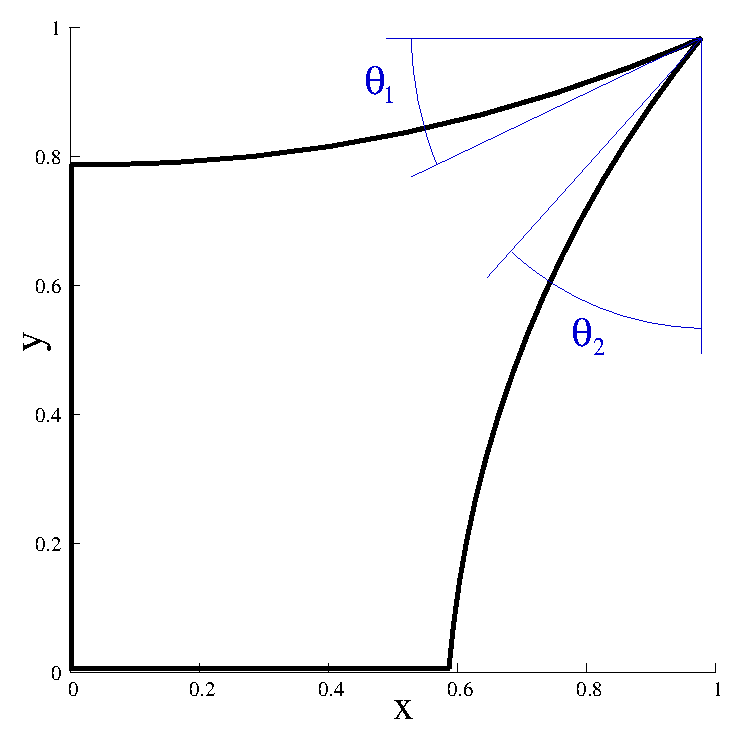
\includegraphics[width=0.3\textwidth]{figs/domains/qugrs_fig.eps}
    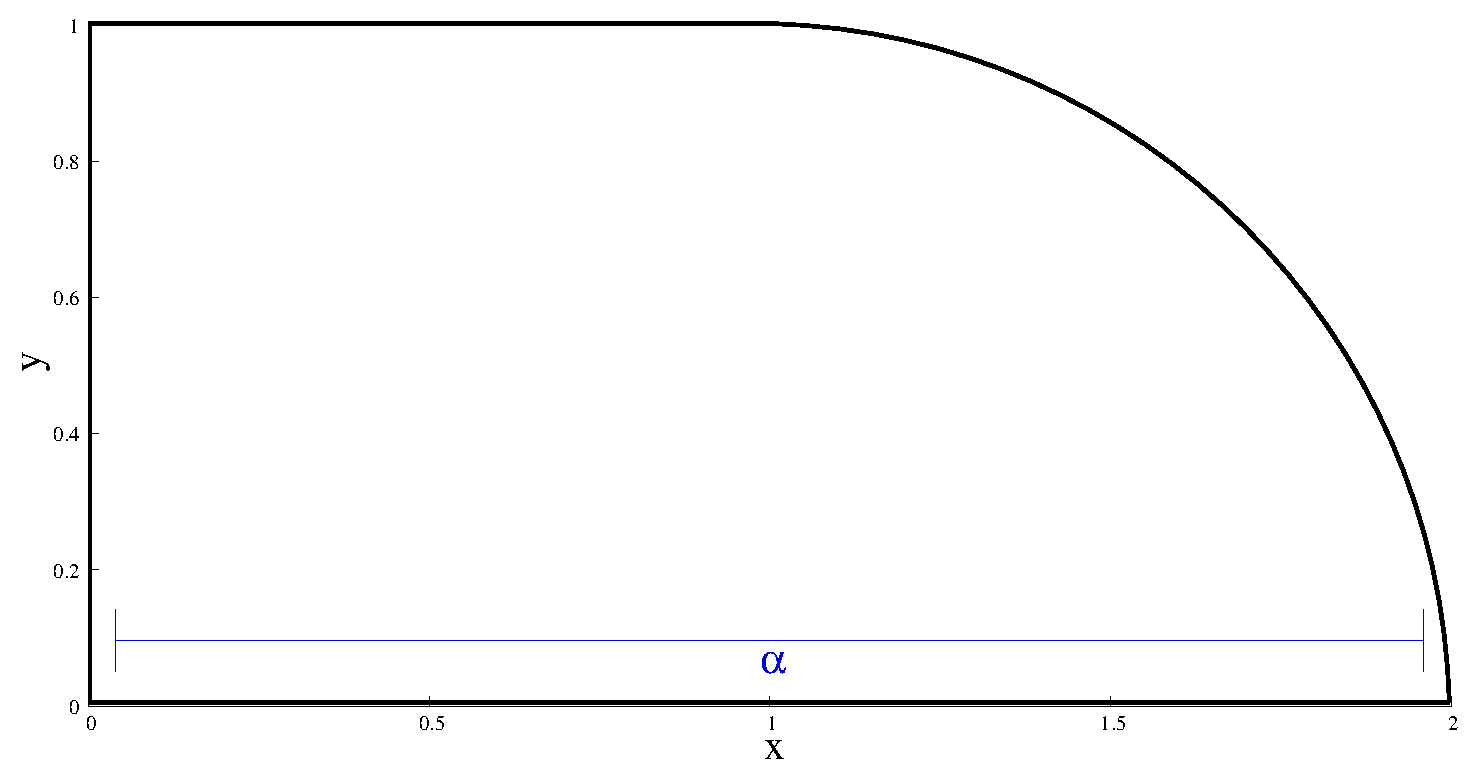
\includegraphics[width=0.6\textwidth]{figs/domains/qust_fig.eps}
    \caption{Left: quarter generalized rectangular Sinai billiard; right: quarter stadium billiard}
    \label{fig:billiards}
  \end{center}
\end{figure}

The Sinai billiard is constructed from circular arcs which meet at $(1,1)$ and is parameterized by two angles, $\theta_{1}$ and $\theta_{2}$, which are the angles from horizonal and vertical of the arcs at $(1,1)$. The Sinai billiard is said to demonstrate ``hard chaos'' becase there are no stable orbits.

The stadium billiard is construced from a rectangular region and a quarter circle and is parameterized by the the horizontal length of the billiard $\alpha$. Trajectories with vertical momentum in the rectangular region are stable but such orbits occupy a measure zero subset of phase space and the quarter stadium still demonstrates chaotic properties.


\chapter{Methods}
\section{Scaling Method}
Vergini and Saraceno \cite{vergini} developed a method of computing high energy eigenfunctions of chaotic billiards using a scaling method. The method simultaneously finds all eigenfunctions $\phi_{i}(\rr)$ with energy in a given window $[E - \Delta E, E + \Delta E]$ by scaling each eigenfunction. The scaled eigenfunctions $\chi_{i}(k, \rr)$ are computed as
\[
\chi_{i}(k, \rr) = \phi_{i} \left( \frac{k}{k_{i}} \rr \right) = \phi_{i} \left( \rr + \frac{\omega_{i}}{k_i} \rr \right)
\]
where $\omega_{i} = k - k_i$. This scaling causes all eigenfunctions to fall approximately in a linear subspace of a single basis set $\left\{ \xi_{l} \right\}_{l=1}^{B}$, that is
\[
\chi_{i}(k, \rr) = \sum_{l=1}^{B} X_{li} \xi_{l}(k, \rr) + \epsilon_{i}(\rr)
\]
where $\epsilon_{i}(\rr) \ll 1$ for sufficiently large $B$. Values of B of approximately $1.5 \frac{k \vert \Gamma \vert}{\pi}$ have been shown to produce $\epsilon < 10^{-4}$. This fact provides a significant efficiency gain over prior methods because many eigenfunctions can be found by solving a single linear system. The basis functions $\xi_{l}(k, \rr)$ depend on the billiard shape being used.For the quarter generalized rectangular Sinai billiard the basis set consists of irregular Bessel functions (which satisfy $(\nabla^{2} + k^2)\xi_{l}(k, \rr) = 0$) placed along $\Gamma^{+}$, the set of points ouside $\Omega$ whose nearest distance to $\Gamma$ is $D$ where $kD$ is taken to be $7$ so that $D$ is appriximately one wavelength. For the quarter stadium, the basis set is plane waves with orientations evently spaced around the circle. The scaling method runs in $O(B^{3})$ time where  is the number of basis functions used. The scaling method only computes coefficients of basis functions which can then be used to evaluate the eigenfunctions at arbitrary $\rr \in \Omega$. \cite{barnett}

\section{Counting Nodal Domains}
Nodal domains are counted by exploring domains pixel by pixel, marking each pixel as ``counted'' once it has been seen. The searching algorithm usded to explore each domain is a hybrid depth- and breadth-first method where for each pixel, the sign of each neighboring pixel is compared to the sign of the nodal domain and if the sign matches, the neighboring pixel is pushed onto a stack. Exploration then continues by popping a pixel off of the stack. This method was chosen so that the signs of all four neighbors (above, below, right, and left) are known when that pixel is being examined, which is necessary for the adaptive interpolation scheme described below.

Letting $N$ be the number of points the eigenfunction is sampled at, this method has computational complexity $O(N)$. This is because the method performs a fixed number of comparisons for each pixel plus $O(N)$ total comparisons searching for an unseen nodal domain after a nodal domain has been explored. This algorithm uses an array of $N$ integers to store, for each pixel, whether it has been counted, which nodal domain it is in, whether or not it is within the boundary of the billiard, and additional information relating to the interpolation method described below. In addition, this method uses a dynamically sized array as a stack whose size it as most the size of the nodal domain being explored and usually only a fraction of that.

\section{Interpolation}
Because sampling eigenfunctions is expensive, we are limited by $N$ which scales like $\Delta x ^{-2}$. As a consequence of working with relatively coursely sampled grids we encounter scenarios where the connectivity of nodal domains is ambiguous (Fig. \ref{fig:interpolation_sample}).

\begin{figure}[h!]
  \begin{center}
    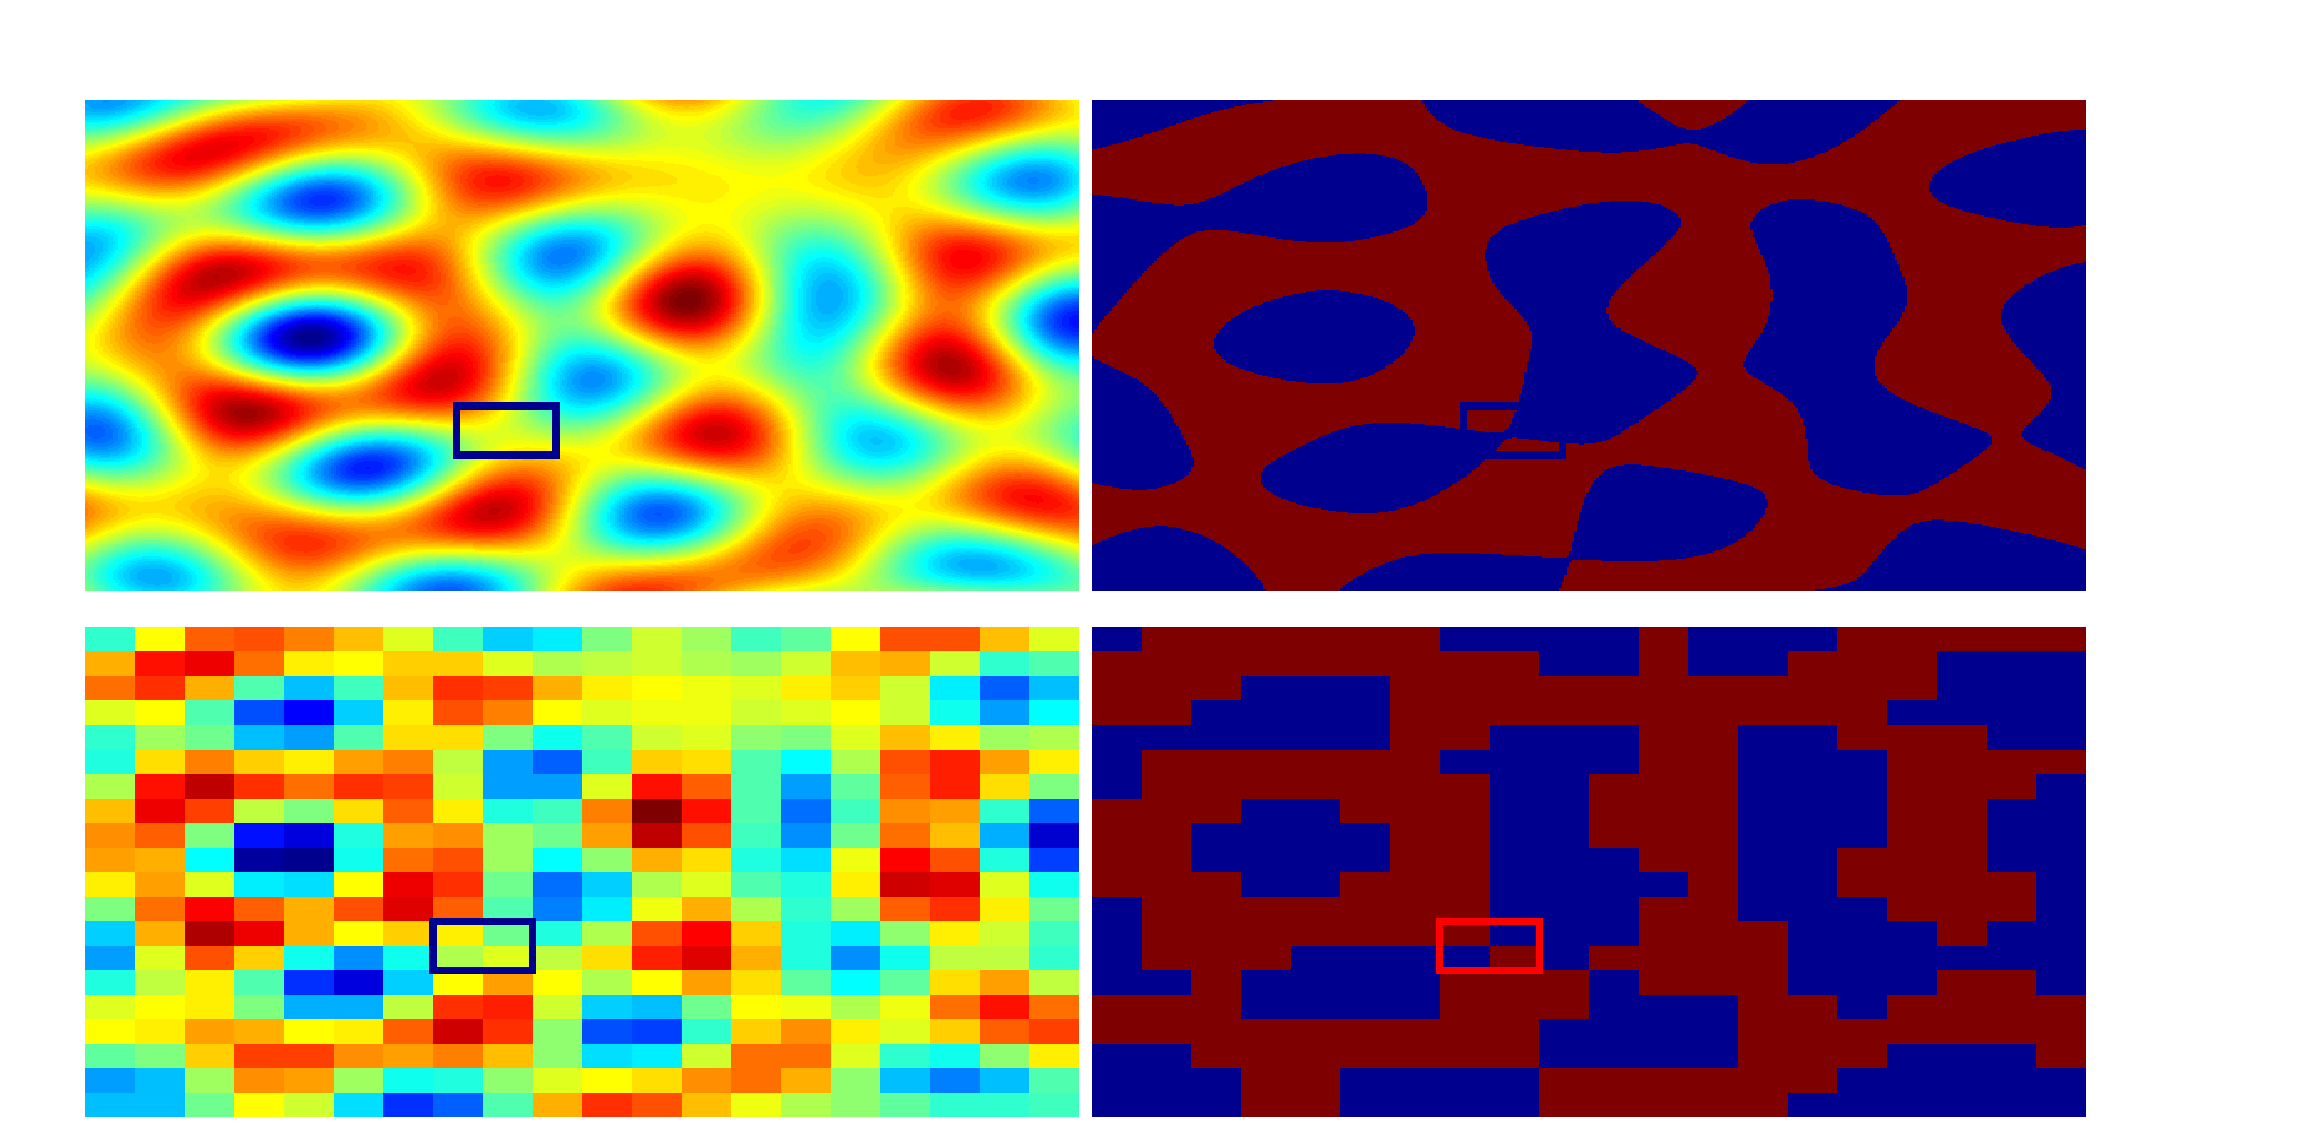
\includegraphics[width=0.9\textwidth]{figs/interpolation_sample.eps}
    \caption{An ambiguity in nodal domain connectivity due to coarse sampling. The ambiguous region is shown with a red box. Top left: high resolution image of an eigenfunction; top right: nodal domains of the same eigenfunction; bottom left: low resolution image of the same eigenfunction; bottom right: nodal domains of low resolution eigenfunction}
    \label{fig:interpolation_sample}
  \end{center}
\end{figure}

We resolve such ambiguities by performing an interpolation in the ambigious region. We interpolate with the functions
\[
J_{n}(\alpha r) \sin(n \theta)
\]
and
\[
J_{n}(\alpha r) \cos(n \theta)
\]
where $J_{n}(r)$ is a regular Bessel function. These functions form a complete orthonormal basis for solutions of (\ref{eq:helmholtz}) (see \ref{sec:helmholtz_basis}). We fix a value $M$ to be the order of the highest order Bessel function, restricting our basis to the finite set
\begin{equation}
  \label{eq:interp_functions}
  \xi_{i}(r, \theta)=\begin{cases}
  J_{i}(\alpha r) & \text{if }i=0\\
  J_{i}(\alpha r)\sin(i\theta) & \text{if }1 \le i \le M\\
  J_{i-M}(\alpha r)\cos((i-M)\theta) & \text{if }M+1 \le i \le 2M
  \end{cases}
\end{equation}
We construct a surrogate function
\[
  \tilde{u}(\rr) = \sum_{i=0}^{2M+1} c_{i} \xi_{i}(\rr)
\]
as a local approximation to the eigenfunction $u(\rr$ by fitting the coeffiecients $c_{i} \in \mathbb{R}$ to minimize the error $\Vert u - \tilde{u} \Vert_{2}$. This function can then be sampled at a higher resolution within the region in question. We define the sampling ratio of this surrogate function to the original eigenfunction to be $\rho$.

Interpolation occurs only between four pixels but uses surrounding values to fit the coefficients $c_i$. The selection of which surrounding values to use is termed a stencil. After testing various stencil shapes we selected one using 24 points consisting of a four by four square with two additional points on each side of the square. See \ref{sec:params} for a discussion of the choice of stencil, $M$, and $\alpha$.

We can construct a single matrix to transform values on a stencil to upsampled values in the center of the stencil, performing the process described above with a single matrix multiplication. We construct the interpolation matrix as
\[
U = L H^{+}
\]
Where $L$ is a matrix which performs an evaluation of Bessel functions at low resolution, $H$ performs an evalution of Bessel functions at high resolution and $A^{+}$ denotes the pseudoinverse of $A$. Specifically,
\[
L_{ij} =\begin{cases}
J_{j}(r_{i}) & \text{for } j = 0 \text{ and } 0 \le i < 24\\
J_{j}(r_{i}) \sin{(j \theta_{i})} & \text{for } 1 \le j \le M \text{ and } 0 \le i < 24\\
J_{j-M}(r_{i}) \cos{((j-M) \theta_{i})} & \text{for } M+1 \le j \le 2M+1 \text{ and } 0 \le i < 24
\end{cases}
\]
and
\[
U_{ij} =\begin{cases}
J_{j}(r_{i}) & \text{for } j = 0 \text{ and } 0 \le i < \gamma\\
J_{j}(r_{i}) \sin{(j \theta_{i})} & \text{for } 1 \le j \le M \text{ and } 0 \le i < \gamma\\
J_{j-M}(r_{i}) \cos{((j-M) \theta_{i})} & \text{for } M+1 \le j \le 2M+1 \text{ and } 0 \le i < \gamma
\end{cases}
\]
where $\gamma = (\rho + 1)^{2}$, $(r_{i},\theta_{i}) = \rr_{i}$ in polar coordinates, and $\rr_{i}$ are points in the stencil.

The pseudoinverse $H^{+}$ is computed using a singular value decomposition as follows,
\[
H^{+} = V \Sigma^{+} U^{*}
\]
where $H = U^{*} \Sigma V$ is a singular value decompostion of $H$ and
\[
\Sigma^{+}_{i,i} =\begin{cases}
\Sigma_{i,i}^{-1} & \text{if }\Sigma_{i,i} > \epsilon\\
\Sigma_{i,i} & \text{otherwise}
\end{cases}
\]
where $\epsilon = \gamma \epsilon_{double} \vert \Sigma \vert$ where $\epsilon_{double}$ is the difference between $1$ and the smallest IEEE double precision floating point number greater than $1$. Singular values less than $\epsilon$ are considered to be zero within working precision.

\chapter{Results}

\appendix
\chapter{General Solution of the Helmholtz Equation}
\label{sec:helmholtz_basis}
Here we show that the functions $J_{n}(\alpha r) \sin(n \theta)$ and $J_{n}(\alpha r) \cos(n \theta)$ for a complete orthonormal basis of solutions of (\ref{eq:helmholtz}).

In polar coordinates,
\[
\nabla^{2} = \frac{1}{r} \partial_{r} (r \partial_{r}) + \frac{1}{r^{2}} \partial_{\theta \theta}
\]
Thus, (\ref{eq:helmholtz}) can be expressed as
\[
u_{rr}(r, \theta) + \frac{1}{r} u_{r}(r, \theta) + \frac{1}{r^{2}} u_{\theta \theta}(r, \theta) + k^2 u(r, \theta) = 0
\]
Using separation of variables we attempt solutions of the form
\[
u(r, \theta) = R(r) \Theta(\theta)
\]
where $\Theta(\theta)$ is periodic with period $2 \pi$. This gives
\[
\Theta''(\theta) + n^{2} \Theta(\theta) = 0
\]
and
\[
r^{2} R''(r) + r R'(r) + r^{2} k^{2} R(r) - n^{r} R(r) = 0
\]
The periodicity of $\Theta(\theta)$ requires that
\[
\Theta(\theta) = \alpha \sin(n \theta) + \beta \cos(n \theta)
\]
where $n \in \mathbb{Z}$.
The radial differential equation is known as Bessel's equation and has solutions
\[
R(r) = J_{n}(k r)
\]
where $k \in \mathbb{R}$ is allowed to take discrete values determined by boundary conditions.

Thus, the general solution of (\ref{eq:helmholtz}) can be expressed as a sum of terms of the form
\[
J_{n}(k r) \sin(n \theta) \text{ and } J_{n}(k r) \cos(n \theta)
\]

\chapter{Interpolation Parameter Selection}
\label{sec:params}
In this section, we discuss the various stencils, $M$, and $\alpha$ values that were considered and how we picked our particular values.
Only stencil shapes that which are symmetric about the four central points were considered. The four shapes considered are shown in figure \ref{fig:stencils}. The most important consideration in choosing a stencil was the accuracy of the interpolation. The size of the stencil affects the computational cost of interpolation but this difference is trivial.

\begin{figure}[h!]
  \begin{center}
    
\includegraphics[width=0.2\textwidth]{figs/stencils/4x4_no_corners_centered.eps}
    \hspace{1.1 cm}
    
\includegraphics[width=0.2\textwidth]{figs/stencils/4x4_centered.eps}
    \linebreak
    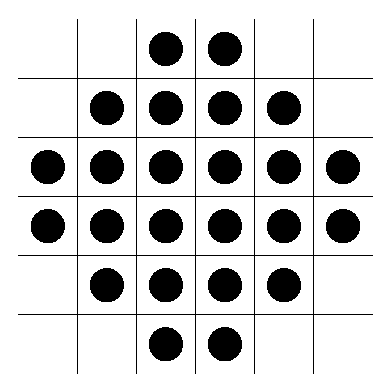
\includegraphics[width=0.3\textwidth]{figs/stencils/4x4+2_centered.eps}
    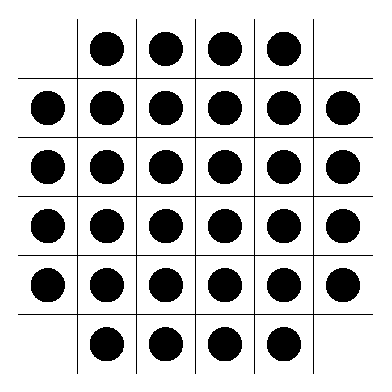
\includegraphics[width=0.3\textwidth]{figs/stencils/6x6_no_corners_centered.eps}
    \caption{The four stencil shapes considered for interpolation}
    \label{fig:stencils}
  \end{center}
\end{figure}

The accuracy of interpolation also depends on $M$ and $\alpha$, which must be considered simultaneously with the choice of stencil. Figure \ref{fig:errors_all} shows a comparison of the infinity norm of the interpolation error over various values of $M$ and $\alpha$ for each of the stencils shown above.

\begin{figure}[h!]
  \begin{center}
    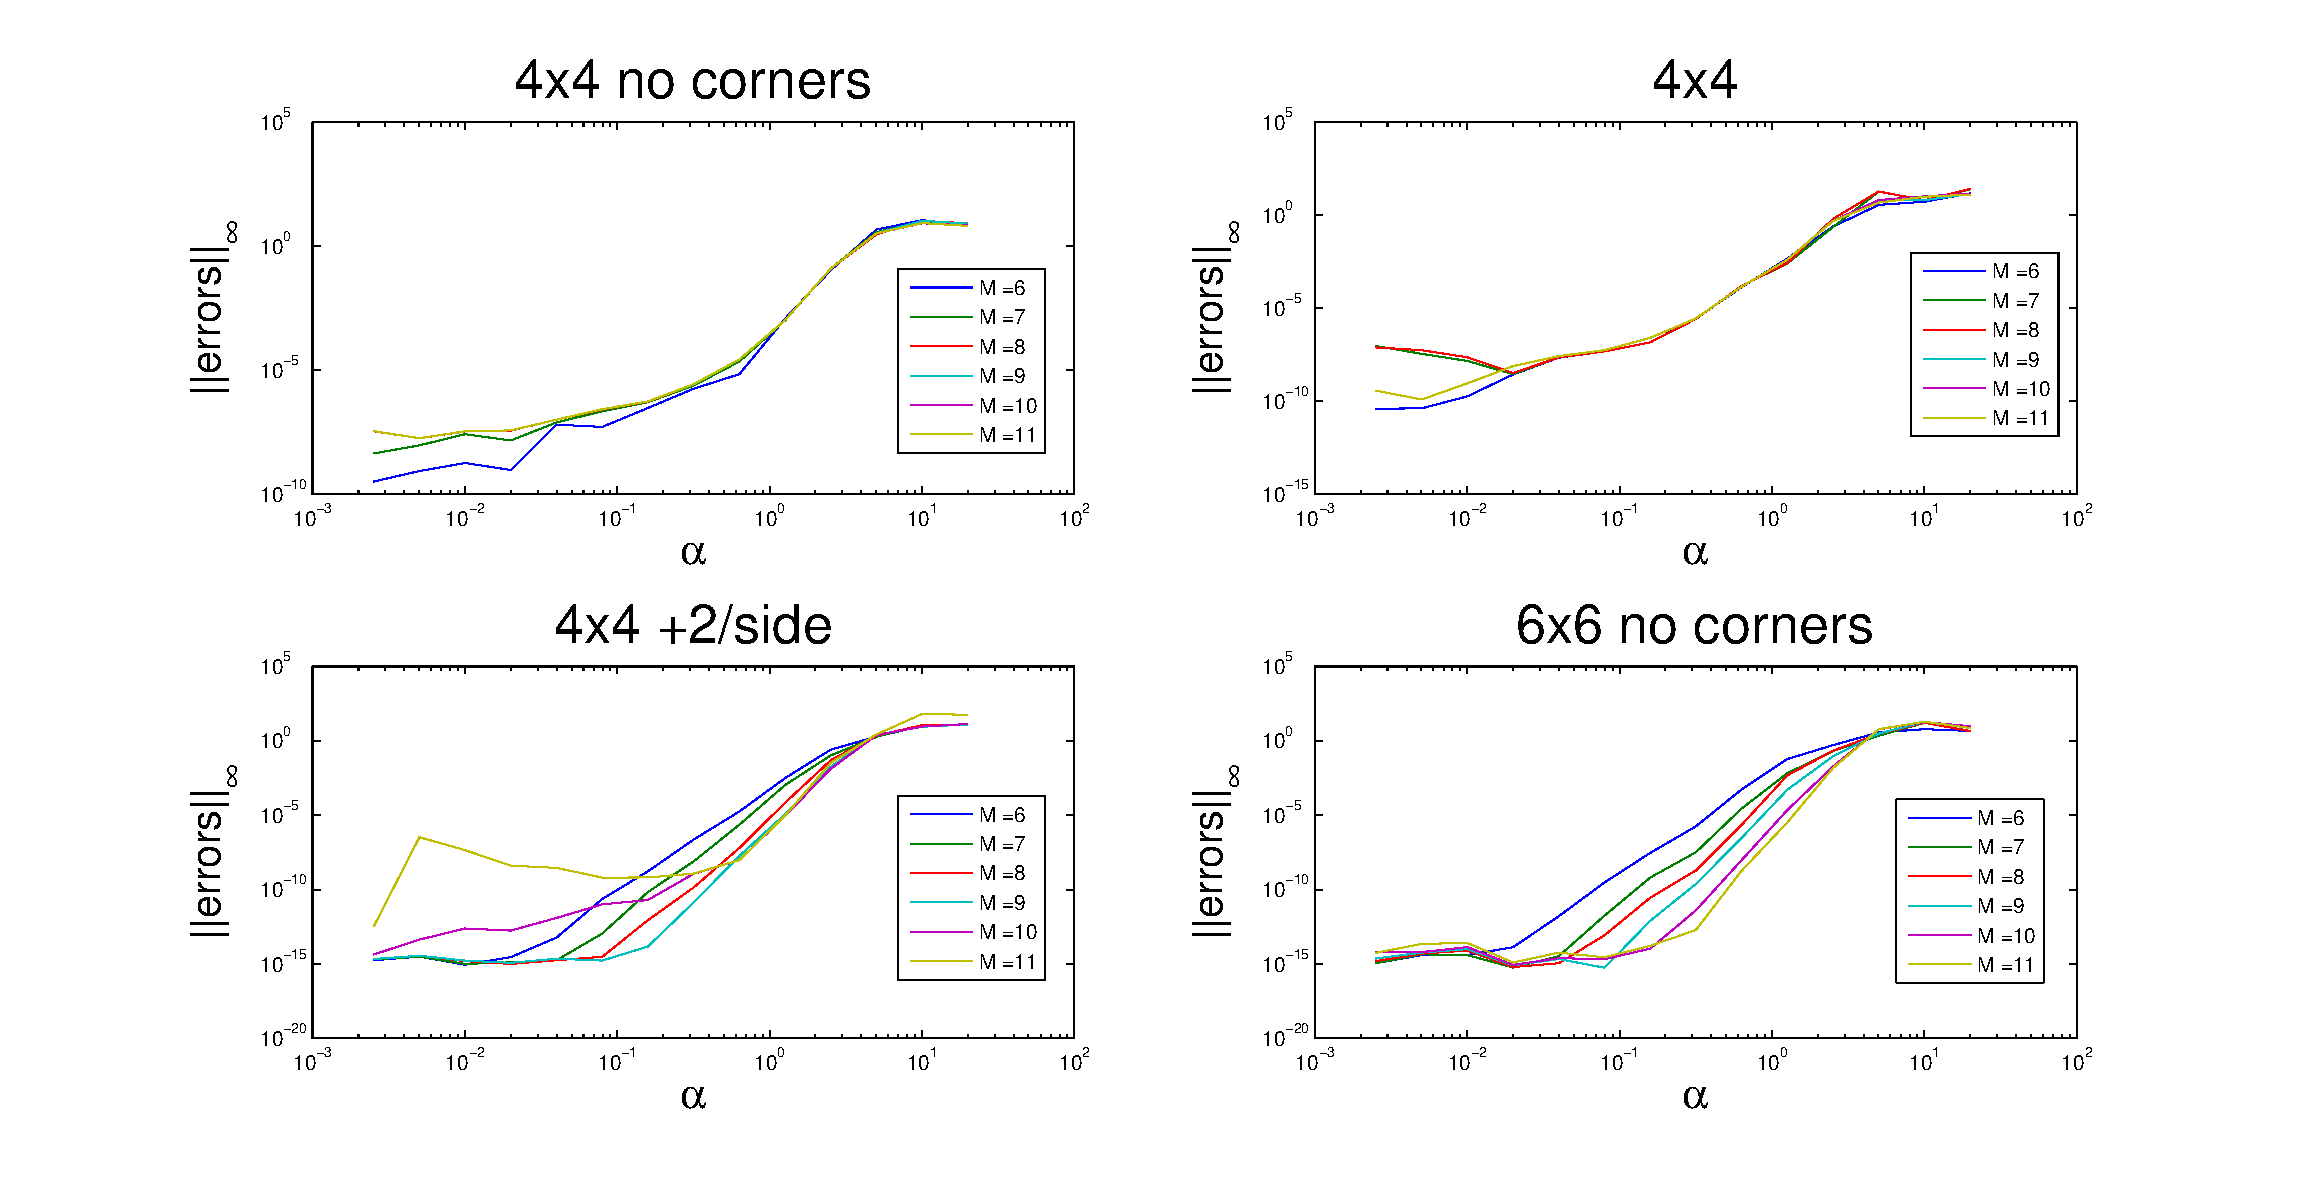
\includegraphics[width=1.2\textwidth]{figs/interpolation/error_norms_all.eps}
    \caption{Comparison of interpolation error norms over $M$ and $\alpha$ for each stencil.}
    \label{fig:errors_all}
  \end{center}
\end{figure}


\bibliographystyle{plain}
\bibliography{thesis}

\end{document}
